% vim: set ft=plaintex:

\documentclass[]{article}
\usepackage{showlabels}

\usepackage[margin=1in]{geometry}
\usepackage{fancyhdr}
\pagestyle{fancy}

\usepackage{amsmath}
\usepackage{mathtools}
\usepackage{amsfonts}
\usepackage{amssymb}
\usepackage{bbm}

\usepackage{braket}
\usepackage[bold]{hhtensor}
\usepackage{cancel}

\usepackage{amsthm}

% load thmtools but fix "proof proof" bug with thmbox
\usepackage{letltxmacro}
\LetLtxMacro\amsproof\proof
\LetLtxMacro\amsendproof\endproof

\usepackage{thmtools}

\AtBeginDocument{%
  \LetLtxMacro\proof\amsproof
  \LetLtxMacro\endproof\amsendproof
}

\usepackage{nameref,hyperref}
\usepackage[capitalize]{cleveref}

\usepackage{natbib}
\bibliographystyle{humannat}
\usepackage[nottoc]{tocbibind}
\usepackage[toc,page]{appendix}

% % show labels for \ref in margins
% \usepackage{seqsplit}
% \usepackage{showkeys}
% \usepackage{xstring}
% \renewcommand*\showkeyslabelformat[1]{%
% \noexpandarg%
% % instead of \textvisiblespace you can also put in ~
% % if you want to keep a plain space at space characters
% \StrSubstitute{\(\{\)#1\(\}\)}{ }{\textvisiblespace}[\TEMP]%
% \parbox[t]{\marginparwidth}{\raggedright\normalfont\small\ttfamily\expandafter\seqsplit\expandafter{\TEMP}}}


\usepackage{algorithm2e}
\usepackage{booktabs}
\usepackage{enumitem}
\usepackage{float}
\usepackage{graphicx}
\usepackage[all]{xy}

\usepackage{comment}
\usepackage{todonotes}

% bold \emph
\let\emph\relax
\DeclareTextFontCommand{\emph}{\bfseries\em}

\declaretheorem[thmbox=M]{theorem}
\declaretheorem[thmbox=M,sibling=theorem]{proposition}
\declaretheorem[thmbox=M,sibling=theorem]{lemma}
\declaretheorem[thmbox=M,sibling=theorem]{corollary}
\declaretheorem[thmbox=M,sibling=theorem]{conjecture}
\declaretheorem[
    thmbox={style=M,bodystyle=\normalfont},
    sibling=theorem,
]{definition}
\declaretheorem[
    thmbox={style=M,bodystyle=\normalfont},
    sibling=theorem,
]{example}
\declaretheorem[style=remark,sibling=theorem]{remark}


\makeatletter
\newcommand{\myref}[1]{\cref{#1}\mynameref{#1}{\csname r@#1\endcsname}}
\newcommand{\Myref}[1]{\Cref{#1}\mynameref{#1}{\csname r@#1\endcsname}}
\def\mynameref#1#2{%
  \begingroup
    \edef\@mytxt{#2}%
    \edef\@mytst{\expandafter\@thirdoffive\@mytxt}%
    \ifx\@mytst\empty\else
    \space(\nameref{#1})\fi
  \endgroup
}
\makeatother

\newcommand{\simiid}{\overset{\text{iid}}{\sim}}
\newcommand{\eps}{\varepsilon}
\newcommand{\Rad}{\text{Rad}}


\newcommand{\NN}{\mathbb{N}}
\newcommand{\ZZ}{\mathbb{Z}}
\newcommand{\CC}{\mathbb{C}}
\newcommand{\RR}{\mathbb{R}}
\newcommand{\TT}{\mathbb{T}}
\newcommand{\ind}{\mathbbm{1}}
\newcommand{\fm}{\mathfrak{m}}

\newcommand{\cA}{\mathcal{A}}
\newcommand{\cB}{\mathcal{B}}
\newcommand{\cD}{\mathcal{D}}
\newcommand{\cE}{\mathcal{E}}
\newcommand{\cG}{\mathcal{G}}
\newcommand{\cH}{\mathcal{H}}
\newcommand{\cL}{\mathcal{L}}
\newcommand{\cM}{\mathcal{M}}
\newcommand{\cN}{\mathcal{N}}
\newcommand{\cO}{\mathcal{O}}
\newcommand{\cF}{\mathcal{F}}
\newcommand{\cK}{\mathcal{K}}
\newcommand{\cS}{\mathcal{S}}
\newcommand{\cU}{\mathcal{U}}
\newcommand{\cX}{\mathcal{X}}

\newcommand{\mX}{\matr{X}}
\newcommand{\mY}{\matr{Y}}
\newcommand{\mA}{\matr{A}}
\newcommand{\mB}{\matr{B}}
\newcommand{\mD}{\matr{D}}
\newcommand{\mI}{\matr{I}}
\newcommand{\mK}{\matr{K}}
\newcommand{\mL}{\matr{L}}
\newcommand{\mM}{\matr{M}}
\newcommand{\mP}{\matr{P}}
\newcommand{\mQ}{\matr{Q}}
\newcommand{\mS}{\matr{S}}
\newcommand{\mU}{\matr{U}}
\newcommand{\mV}{\matr{V}}
\newcommand{\mZ}{\matr{Z}}
\newcommand{\mSigma}{\matr{\Sigma}}
\newcommand{\mLambda}{\matr{\Lambda}}
\newcommand{\va}{\vec{a}}
\newcommand{\vb}{\vec{b}}
\newcommand{\vc}{\vec{c}}
\newcommand{\vf}{\vec{f}}
\newcommand{\vg}{\vec{g}}
\newcommand{\vk}{\vec{k}}
\newcommand{\vmu}{\vec{\mu}}
\newcommand{\vp}{\vec{p}}
\newcommand{\vq}{\vec{q}}
\newcommand{\vu}{\vec{u}}
\newcommand{\vw}{\vec{w}}
\newcommand{\vx}{\vec{x}}
\newcommand{\vy}{\vec{y}}
\newcommand{\vz}{\vec{z}}
\newcommand{\vbeta}{\vec{\beta}}
\newcommand{\vsigma}{\vec{\sigma}}
\newcommand{\vxi}{\vec{\xi}}


\DeclareMathOperator{\id}{id}
\DeclareMathOperator{\im}{im}
\DeclareMathOperator{\Ball}{Ball}
\DeclareMathOperator{\Cov}{Cov}
\DeclareMathOperator{\argmax}{argmax}
\DeclareMathOperator{\argmin}{argmin}
\DeclareMathOperator{\diag}{diag}
\DeclareMathOperator{\Var}{Var}
\DeclareMathOperator{\Tr}{Tr}
\DeclareMathOperator{\rank}{rank}
\DeclareMathOperator{\adj}{adj}
\DeclareMathOperator{\TV}{TV}
\DeclareMathOperator{\Vol}{Vol}
\DeclareMathOperator{\conv}{conv}



\newcommand{\ex}{\mathbb{E}}


\begin{document}

\title{STAT260: Robust Statistics Course Notes}
\author{Feynman Liang\thanks{\texttt{feynman@berkeley.edu}} \\ Department of Statistics, UC Berkeley}
\date{Last updated: \today}

\maketitle

\tableofcontents

\begin{comment}
\end{comment}

\section{9/3/2019}

\begin{figure}[H]
    \centerline{
        \xymatrix{
            \txt{train \\ $\tilde{p}$} \ar[d] \ar@{<->}[r]^-{D(\tilde{p}, p^*) \leq \eps} \ar[dr]
            & \txt{test\\$p^* \in \cG$} \ar[dr] \\
            \txt{$X_1, \ldots, X_n$\\samples} \ar[r] &
            \txt{$\hat\theta(\tilde{p})$\\estimator} \ar[r] &
            \txt{$L(p^*, \hat\theta)$\\loss}
        }
    }
    \caption{Overview of the framework. Training distribution $\tilde{p}$ differs
        from test distribution $p^*$ by some discrepancy $D(\tilde{p}, p^*) \leq \epsilon$.
        We constrain $p^* \in \cG$ to encode distributional assumptions.
        Given an estimator $\hat\theta$ trained using samples $X_1, \ldots, X_n \sim \tilde{p}$,
        we want to control the loss $L(p^*, \hat\theta)$ incurred at test time.
    }\label{fig:robust-statistics-framework}
\end{figure}


\subsection{Minimum distance functional}

Introduced in \cite{donoho1988automatic}, the minimum distance functional is one way to
produce robust estimators which easily generalizes and also leverages distributional assumptions
in $\cG$.

\begin{definition}[Minimum distance functional]\label{def:mdf}
    The \emph{minimum distance functional} (MDF) is
    \begin{align}
        \hat\theta(\tilde{p}) &= \theta^*(q) = \argmin_{\theta} L(q, \theta)
        \text{ where }
        q = \argmin_{q \in \cG} D(\tilde{p}, q)
    \end{align}
    In other words, $q$ is the projection (under $D$) of $\tilde{p}$ onto $\cG$
    and $\hat\theta$ is the estimator obtained by using $q$ as the training distribution.
\end{definition}

One nice property of the MDF is that we can bound it using a supremum over
nearby pairs $p,q \in \cG$ satisfying $D(p,q) \leq 2 \eps$. This is useful
because we eliminate $\tilde{p}$ and focus the theory around $\cG$.
\begin{proposition}[Modulus of continuity bound]\label{prop:mdf-modulus-error-bound}
    If $D$ is a pseudometric (metric without requirement $d(x,y) = 0 \implies x = y$),
    then the cost $L(p^*, \hat\theta(\tilde{p}))$ of the MDF (\cref{def:mdf}) is bounded by:
    \begin{align}
        \fm(\cG, 2\eps, D, L) &= \sup_{\substack{p, q \in \cG \\ D(p,q) \leq 2 \epsilon}} L(p, \theta^*(q))
    \end{align}
    $\fm$ is called the \emph{modulus of continuity}.
\end{proposition}

\begin{proof}
    First fix $p = p^* \in \cG$
    \begin{align}
        \fm \geq \sup_{g \in \cG : D(p^*, q) \leq 2 \epsilon} L(p^*, \theta^*(g))
    \end{align}
    Next, let $q = \argmin_{g \in \cG} D(g, \tilde{p})$ be the projection of $\tilde{p}$ onto $\cG$
    as in \cref{def:mdf}.
    Then since $D(p^*, \tilde{p}) \leq \eps$ by assumption and $p^* \in \cG$, we have
    \begin{align}
        D(q, \tilde{p}) = \min_{g \in \cG} D(g, \tilde{p}) \leq D(p^*, \tilde{p}) \leq \eps
    \end{align}

    The following drawing visualizes the argument.
    \begin{figure}[H]
        \centering
        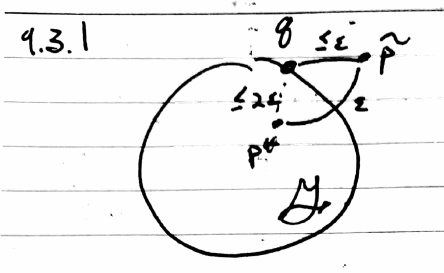
\includegraphics[width=0.7\textwidth]{figures/9-3-1.png}
        \caption{Given $D(p^*, \tilde{p}) \leq \eps$, $p^* \in \cG$, and
            $q$ is the projection of $\tilde{p}$ onto $\cG$ under $D$, we must
            have $D(\tilde{p}, q) \leq \eps$ and by triangle inequality
            $D(p^*, q) \leq 2\eps$
        }
    \end{figure}

    So $D(p^*, q) \leq 2 \eps$ and we can conclude
    \begin{align}
        \fm \geq L(p^*, \theta^*(q))
    \end{align}
\end{proof}

For now, we will specialize to the case $D = \TV$ and $L(p,  \theta) = \|\theta - \mu(p^*)\|_2$.
Consider a Gaussian distributional assumption $\cG_{gauss} = \{\cN(\mu, I) : \mu \in \RR^{d}\}$.

\begin{lemma}\label{lem:gauss-tv}
    $\TV(\cN(\mu, I), \cN(\mu', I)) \asymp \Theta(\min(\|\mu - \mu'\|_2, 1))$

    Therefore
    \begin{align}
         \fm(\cG_{gauss}, \eps) = \sup_{\substack{p,q \in \cG\\ \TV(p,q) \leq 2 \eps}} \|\mu(p) - \mu(q)\|_2 = \Theta(\eps)
    \end{align}
    for sufficiently small $\eps$.
\end{lemma}

\begin{proof}
    We first prove the 1D case. By translational symmetry, we can translate both
    distributions while preserving $\|\mu - \mu'\|_2 \eqqcolon u$ so that wlog we may
    assume the two distributions are $p = \cN(\frac{u}{2}, 1)$ and $q = \cN(-\frac{u}{2}, 1)$.
    Then
    \begin{align}
        \TV(p,q)
        &= \frac{1}{2} \frac{1}{\sqrt{2\pi}} \int_{-\infty}^\infty \lvert e^{(t + u/2)^2/2} - e^{(t-u/2)^2/2}\rvert dt \\
        &= \frac{1}{\sqrt{2\pi}} \int_{-u/2}^{u/2} e^{-t^2/2} dt \label{eq:9-3-int}
    \end{align}
    where the last equality follows by cancelling the probability mass in the following picture:
    \begin{figure}[H]
        \centering
        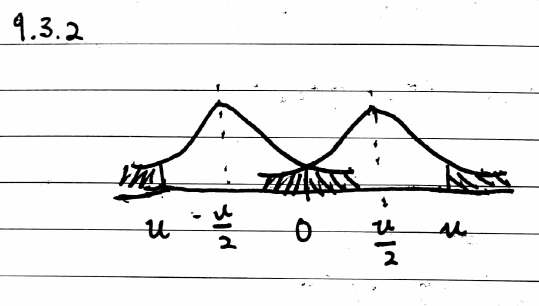
\includegraphics[width=0.7\textwidth]{figures/9-3-2.png}
        \caption{Both Gaussians exhibit identical $\pm \frac{u}{2}$ tails with opposite signs
            in the expression for $\TV$, so the $\TV$ is equivalent to the area in $[-u/2, u/2]$ drawn
            out by the pointwise max between the two PDFs. By symmetry, this is just twice the area
            inside $[-u/2, u/2]$ which after cutting and pasting integration areas (and cancelling the $1/2$
            in definition of $\TV$) is equal
            to the probability mass between $[-u/2,u/2]$ for a Gaussian.}
    \end{figure}

    Note that $e^{-t^2/2} \geq \frac{1}{2}$ if $\lvert t \rvert < 1$, so $\TV = \Omega(\min(u,1))$
    which can be seen by splitting the integral and examining the two cases where
    $\frac{u}{2} > 1$ (which yields the $1$) and $\frac{u}{2} < 1$ (which yields the $u$).

    Similarly, $e^{-t^2/2} \leq 1$ for all $t > 0$ so $\TV = O(\min(u,1))$.

    To generalize to higher dimensions, note identity covariance implies rotational invariance so we can
    rotate and translate such that the two means are on the first coordinate axis and separated
    by $\|\mu - \mu'\| = \lvert \mu_1 - \mu_1' \rvert$. In particular, $\mu_i = 0$ for $i \neq 1$ hence
    in the $\TV$ expression they can be factored out and integrated to $1$ to reduce to the 1D case.
\end{proof}

\subsection{Midpoint lemma and resilience}

As a less restrictive family, consider distributions with bounded covariance:
\begin{align}
    \cG_{cov}(\sigma)
    &= \{ p : \ex_p[(X - u)(X - u)'] \preceq \sigma^2 I\}
\end{align}

We begin with an important lemma which will be used to prove the modulus of continuity for $\cG_{cov}$
and generalized in the following section.
\begin{lemma}[Midpoint lemma]\label{lem:midpoint}
    If $\TV(p,q) \leq \eps$ then exists a \emph{midpoint} distribution $r$ such that
    $r \leq \min\{\frac{p}{1 - \eps}, \frac{q}{1 - \eps}\}$ and
    \begin{enumerate}
        \item $r(x) \leq \frac{p(x)}{1 - \eps}$ for all $x$
        \item $r$ is an \emph{$\epsilon$-deletion of $p$} (obtained by deleting $\epsilon$ mass from $p$)
        \item $r = p \vert_{E}$ for $p(E) \geq 1 - \eps$ where $E \mid X$ has probability $1$ if $p(x) \leq q(x)$ and $\frac{q(x)}{p(x)}$ if $p(x) > q(x)$
    \end{enumerate}
\end{lemma}

\begin{proof}
    The midpoint distribution is given by $r = \frac{\min(p,q)}{1 - \TV(p,q)}$ and is obtained from $p$
    by deleting probability mass from $q$ and renormalizing.
    \begin{figure}[H]
        \centering
        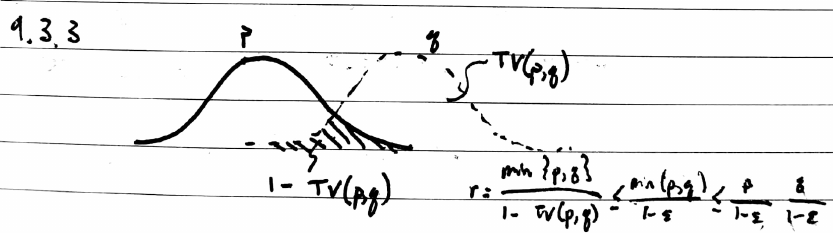
\includegraphics[width=0.6\textwidth]{figures/9-3-3.png}
        \caption{The midpoint distribution $r = \frac{\min(p,q)}{1 - \TV(p,q)}$ can be reached
        from both $p$ and $q$ by deleting $\epsilon$-mass and renormalizing.}
    \end{figure}
    Specifically, we delete
    $q(x) - p(x)$ mass from all points in $\{ x : q(x) > p(x) \}$, the integral of which is precisely
    equal to the total variation distance. This means that we must renormalize by $1 - \eps$ to ensure
    $r$ is a proper distribution.
\end{proof}

\begin{corollary}\label{corr:mod-cont-cov}
    $\fm(\cG_{cov}(\sigma), \eps) = O(\sigma \sqrt{\eps})$
\end{corollary}

\begin{proof}
    Take $p, q \in \cG_{cov}$ such that $\TV(p, q) \leq \eps$.
    By \cref{lem:midpoint}, there exists a midpoint distribution
    $r = p \mid_E$ for which
    \begin{align}
        \ex_r[X - \mu(p)]
        &= \ex_p[X - \mu(p) \mid \underbrace{E}_{1 - \eps}]
        = \frac{-\eps}{1 - \eps} \ex_p[X - \mu(p) \mid \underbrace{E^c}_{\eps}]
    \end{align}
    where the last equality follows from
    \begin{align}
        0
        &= \ex_p[X - \mu(p)]
        = \underbrace{p(E)}_{1-\epsilon} \ex_p[ X - \mu \mid E] + \underbrace{p(E^c)}_{\epsilon} \ex_p[X - \mu \mid E^c]
    \end{align}
    (This is a common trick for moving from conditioning on an event to
    conditioning on its complement in zero mean functionals).

    (Chebyshev in $\RR^d$) By linearity of expectation and Jensen's inequality
    \begin{align}
        \| \ex_p[X - \mu(p) \mid E^c] \|_2
        &= \sup_{\|v \|_2 \leq 1} \braket{\ex_p[X - \mu(p) \mid E^c], v} \\
        &= \sup_{\|v\|_2 \leq 1} \ex_p [\braket{X - \mu(p), v} \mid E^c] \\
        &\leq \sup_{\|v \|_2 \leq 1} \sqrt{\ex_p[\braket{X - \mu(p), v}^2 \mid E^c]}
    \end{align}
    Note $\ex_p[\braket{X - \mu(p), v}^2]
    = \Var_p[\braket{X - \mu(p), v}]
    = v^\top \Cov_p(X) v \leq \sigma^2$ so
    \begin{align}
        \| \ex_p[X - \mu(p) \mid E^c] \|_2
        &\leq \sqrt{\frac{\sigma^2}{\Pr[E^c]}}
        = \frac{\sigma}{\sqrt{\eps}}
        \label{eq:9-3-cheb-cov-control}
    \end{align}
    As a result, we have
    \begin{align}
        \|\mu(r) - \mu(p)\|_2 = \|\ex_r[X - \mu(p)]\|_2 \leq \frac{\eps}{1 - \eps} \frac{\sigma}{\sqrt{\eps}} \leq 2 \sigma \sqrt{\eps}
    \end{align}
    for $\eps < 1/2$.
    A similar argument involving $q$ gives $\|\mu(r) - \mu(q)\|_2 \leq 2 \sigma \sqrt{\eps}$
    so by triangle inequality $\|\mu(p) - \mu(q)\|_2 \leq 4 \sigma \sqrt{\eps}$.
\end{proof}

\begin{remark}
    Unlike the trimmed mean, there is no dependence on $d$ here.
    This means that the MDF remains a good robust estimator even in high dimensions!
\end{remark}

The above proof utilizes two key ingredients:
\begin{itemize}
    \item The midpoint property of $\TV$; both $p$ and $q$ are close to some $\eps$-deletion $r$
    \item The bounded tails (second moment) of $\cG_{cov}$, which is used to control how close $\mu(r)$
    and $\mu(p)$ are in \cref{eq:9-3-cheb-cov-control}
\end{itemize}

The previous proof can be suitably generalized to yield a modulus of continuity bound
for other families:
\begin{definition}[Resilient distribution]\label{def:resilience}
    A distribution is $(\rho, \eps)$-resilient if
    \begin{align}\label{eq:resilience-property}
        r \leq \frac{p}{1 - \eps} \implies \|\ex_r[X] - \ex_p[X]\|_2 \leq \rho
    \end{align}
    In other words, for any (not just midpoint) $\eps$-deletion $r$ the mean does not change in
    norm by more than $\rho$. Equivalently (e.g. when $p$ does not have a density) we can view $r = p \mid_E$
    for an event $E$ and use the definition
    \begin{align}
        p(E) \geq 1 - \eps \implies \|\ex_p[X \mid E] - \ex_p[X]\| \leq \rho
    \end{align}

    We let $\cG_{TV}(\rho, \epsilon)$ be the set of all $(\rho, \epsilon)$-resilient distributions.
\end{definition}

\begin{remark}
    This definition is only applicable for mean estimation under squared error loss.
\end{remark}

\begin{figure}[H]
    \centering
    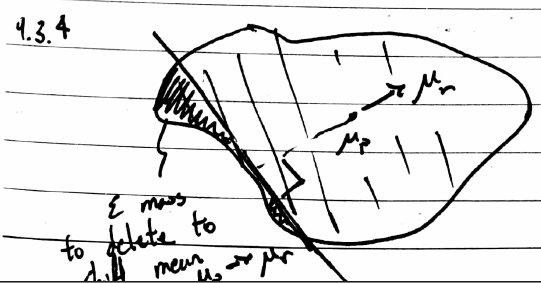
\includegraphics[width=0.5\textwidth]{figures/9-3-4.png}
    \caption{Deleting $\eps$ mass from a resilient distribution $p$ shifts the mean by a controlled
    amount $\|\mu_p - \mu_r\|_2 \leq \rho$.}
\end{figure}

\begin{example}\label{eg:bdd-cov-resilient}
    \cref{corr:mod-cont-cov} shows $\cG_{cov}(\sigma) \subset \cG_{TV}(2 \sigma \sqrt{\eps}, \eps)$
\end{example}

\begin{example}
    \cref{lem:gauss-tv} shows $\cG_{gauss}(\sigma) \subset \cG_{TV}(\eps \sqrt{\log \frac{1}{\eps}}, \eps)$
\end{example}

Combining with \cref{prop:mdf-modulus-error-bound}, for squared error loss we can say
\begin{corollary}[Modulus of continuity bound for resilient distributions]\label{corr:mod-bound-resilient}
    \begin{align}
        \fm(\cG_{TV}(\rho, \eps), \eps) \leq 2 \rho
    \end{align}
\end{corollary}
\begin{proof}
    For any $p,q \in \cG_{\TV}$,
    use \cref{lem:midpoint} to get a midpoint distribution
    and then \cref{eq:resilience-property} with triangle inequality to control the squared error loss.
\end{proof}
So we can always project onto the family of resilient distributions to get a MDF
estimator which has loss independent of $d$.

\subsection{Orlicz norms}

\begin{definition}[Orlitz function / norm]
    An \emph{Orlicz function} $\psi : \RR_{\geq 0} \to \RR_{\geq 0}$ is
    \begin{enumerate}
        \item Convex
        \item Non-decreasing
        \item $\psi(0) = 0$, $\psi(x) \to \infty$ as $x \to \infty$
    \end{enumerate}

    Given an Orlicz function $\psi$, the \emph{Orlicz norm} or $\psi$-norm of a
    random variable $X$ is
    \begin{align}
        \|X\|_\psi &= \inf \left\{t : \ex \psi\left(\frac{\lvert X \rvert}{t} \right) \leq 1 \right\}
    \end{align}
    For multivariate $X \in \RR^d$, define
    \begin{align}
        \|X\|_\psi = \inf \left\{t > 0 : \sup_{v \in \cS^{d-1}} \|\braket{X, v}\|_\psi \leq t \right\}
        \label{def:orlicz-norm-multivar}
    \end{align}
    In other words, $X$ has bounded $\psi$-norm if all of its one dimensional projections do.

    Let $\cG_\psi(\sigma) = \{ X : \|X - \ex[X]\|_\psi \leq \sigma \}$.
\end{definition}

\begin{example}
    $\psi(x) = x^k$ gives $\|X\|_\psi = \left(\ex[\lvert X \rvert^k]\right)^{1/k}$,
    which looks like $L_p$ norms. In fact, these are precisely distributions with bounded $k$th moments.

    For $\psi(x) = x^2$, we have $\cG_{\psi}(\sigma) = \cG_{cov}(\sigma)$.
\end{example}

\begin{definition}[Sub-Gaussian/Sub-Exponential]\label{def:sub-gaussian-sub-exp-orlicz}
    For $\psi_2(x) = e^{x^2} - 1$, $\cG_{\psi_2}(\sigma)$ are called the $\sigma$-sub-Gaussian random variables.

    For $\psi_1(x) = e^x - 1$, $\cG_{\psi_1}(\sigma)$ are called the $\sigma$-sub-exponential random variables.
\end{definition}

The next proposition shows that any distribution with bounded Orlicz norm is resilient.
\begin{proposition}[Bounded Orlicz norm implies resilience]\label{lem:orlicz-norm-resilient}
    $\cG_{\psi}(\sigma) \subset \cG_{TV}(2 \sigma \eps \psi^{-1}(\frac{1}{\eps}), \eps)$
    if $\eps < 1/2$.

    $\psi(x) \to \psi^{-1}(x) = \sqrt{x} \to \eps \psi^{-1}(1/\eps) = \sqrt{\eps}$
\end{proposition}

\begin{proof}
    \begin{align}
        \|\ex_r[X] - \ex_p[X]\|_2
        &= \|\ex_p[X - \mu \mid \underbrace{E}_{p(E) = 1 - \eps} ]\|_2
        = \frac{\eps}{1 - \eps} \| \ex_p [ X- \mu \mid E^c] \|
    \end{align}
    Focusing in on the expectation term
    \begin{align}
        \| \ex_p[X - \mu \mid E^c] \|_2
        &= \sup_{\|v\|_2 = 1} \ex_p[\braket{X - \mu, v} \mid E^c]
    \end{align}
    By Jensen's inequality, convexity of $\psi$ (equivalently concavity of $\psi^{-1}$),
    definition of multivariate Orlicz norm (\cref{def:orlicz-norm-multivar}),
    and monotonicity of $\psi$, we have
    \begin{align}
        \| \ex_p[X - \mu \mid E^c] \|_2
        &= \sup_{\|v\|_2 = 1} \sigma \left(
            \ex_p\left[(\sigma \psi^{-1} \circ \psi)\left( \frac{\lvert \braket{X - \mu, v} \rvert}{\sigma} \right) \mid E^c\right]
        \right) \\
        &\leq \sup_{\|v\|_2 = 1} \sigma \psi^{-1}\left(
            \ex_p\left[\psi\left( \frac{\lvert \braket{X - \mu, v} \rvert}{\sigma} \right) \mid E^c\right]
        \right) \\
        &\leq \sup_{\|v\|_2 = 1} \sigma \psi^{-1}\left(
            \underbrace{\ex_p\left[\psi\left( \frac{\lvert \braket{X - \mu, v} \rvert}{\sigma} \right) \right]}_{\leq 1}
            \underbrace{\frac{1}{\Pr[E^c]}}_{\frac{1}{\eps}}
        \right) \\
        &\leq \sigma \psi^{-1}(\frac{1}{\eps})
    \end{align}
\end{proof}

\section{9/5/2019}

\subsection{Recap}

\begin{itemize}
    \item Minimum distiance functionals: good error, bounded by modulus of continuity $\fm$
    \item Resilience $\implies$ bounded $\fm$
    \item Bounded Orlicz $\psi$-norm $\implies$ resilience
\end{itemize}
This lecture:
\begin{itemize}
    \item Want to analyze $X_1, \ldots, X_n$
    \item ``The empirical average converges to the mean if $n$ is large''
    \item Two steps:
    \begin{enumerate}
        \item Show \emph{concentration inequality}: bound variation of $p$ in terms of $\sigma$
        \item Show \emph{composition property}: $\sigma$ gets smaller as we take more independent samples
    \end{enumerate}
\end{itemize}

\subsection{Concentration Inequalities and Composition}

\begin{example}
    A slot machine has expected payout of \$5 and always pays out positive.
    
    \textbf{Question}: What is the maximum probability of $\geq \$100$?
    
    \textbf{Answer}: 5\%, by letting $P(X=\$0) = 0.95$ and letting $P(X=\$100) = 5\%$.
\end{example}

The preceding example is an instance of \nameref{thm:markov}:
\begin{theorem}[Markov's Inequality]\label{thm:markov}
    If $X \geq 0$ has bounded first moment, then
    \begin{align}
        \Pr[X \geq t \ex[X]] &\leq \frac{1}{t}
    \end{align}
\end{theorem}
\begin{proof}
    \begin{align}  
        t \ex[X] \ind\{X \geq t \ex[X]\} &\leq X
    \end{align}
    Take expectation of both sides and rearrange.
\end{proof}

\nameref{thm:markov} has a nice composition property:
\begin{theorem}[Composition of Markov for sums]\label{thm:markov-composition}
    Let $X_1, X_2 \sim p$ with mean $\mu$.
    \begin{align}
        \Pr\left[ \frac{X_1 + X_2}{2} \geq t \mu \right] &\leq \frac{1}{t}
    \end{align}
\end{theorem}
This is because $\ex[(X_1 + X_2) / 2] = \mu = \ex[X_1] = \ex[X_2]$.

We can apply \nameref{thm:markov} to $Z = f(X)$ for $f : \RR \to \RR_{\geq 0}$
and get a family of inequalities
(provided $\ex[f(X)] < \infty$).
For example, taking $Z = (X - \mu)^2$ and assuming $\ex[Z] = \Var[X] = \sigma^2 < \infty$ yields
\begin{theorem}[Chebyshev's inequality]\label{thm:chebyshev}
    \begin{align}
        \Pr[\lvert X - \mu\rvert \geq t \sigma] \leq \frac{1}{t^2}
    \end{align}
\end{theorem}

Analogous to \myref{thm:markov-composition},
a composition property for \nameref{thm:chebyshev} would require a composition property involving variances:
\begin{theorem}[Variances add for independent RVs]
    If $\{X_i\}_{i=1}^n$ are independent, then
    \begin{align}
        \Var\left[ \sum_{i=1}^n X_i \right] = \sum_{i=1}^n \Var[X_i]
    \end{align}
\end{theorem}

\begin{example}[Concentration of empirical average]
    Let $X_1, \ldots, X_n \simiid p$ with mean $\mu$ and variance $\sigma^2$.
    Let $S = \sum_i^n X_i$ and $\frac{S}{n}$ the empirical average. Then
    \begin{align}
        \Var[S/n] = n \Var[X/n] = n \frac{\sigma^2}{n^2} = \frac{\sigma^2}{n}
    \end{align}
    Hence, the standard deviation of the empirical average $\frac{S}{n}$ is $\sigma_{avg} = \frac{\sigma}{\sqrt{n}}$.
    \nameref{thm:chebyshev} then yields
    \begin{corollary}\label{cor:chebyshev-empirical-avg-concentration}
        \begin{align}
            \Pr\left[
                \left\lvert \frac{S}{n} - \mu \right\rvert \geq t \frac{\sigma}{\sqrt{n}}
            \right] &\leq \frac{1}{t^2}
        \end{align}
    \end{corollary}
\end{example}

The $t^{-2}$ quadratic decay in \cref{cor:chebyshev-empirical-avg-concentration} is tight, as the following
proposition shows:
\begin{proposition}[Lower bounds for Chebyshev]
    There exists $X_1, \ldots, X_n$ pairwise independent, bounded in $[-1, 1]$, mean zero, variance one, such that
    \begin{align}
        \Pr\left[\sum_{i=1}^n X_i = n \right] = \frac{1}{n}
    \end{align}
    Consequently, \cref{cor:chebyshev-empirical-avg-concentration} (with $\mu=0$, $\sigma=1$, and $t = \sqrt{n}$)
    is tight.
\end{proposition}
\begin{proof}
    Flip $k$ independent coins and let $n = 2^k$. For any subset $\emptyset \subsetneq S \subset [k]$, define the random variable
    \begin{align}
        X_S = \begin{cases}
            1 &\text{\# heads in $S$ is even} \\
            -1 &\text{\# heads in $S$ is odd}
        \end{cases}
    \end{align}
    $X_S$ is mean zero, variance one, bounded $[-1,1]$, and pairwise
    independent (since the coin flips are). The event $\{ \sum_{i=1}^n X_i = n \}$
    occurs iff all of the coins land tails, which occurs with probability $2^{-k} = \frac{1}{n}$.
\end{proof}

\subsection{Failure of composition of higher moments and Rosenthal's inequality}\label{ssec:rosenthals-inequality}

To try to extend \nameref{thm:chebyshev}, we can consider applying \nameref{thm:markov} to
$Z = f(X) = (X - \mu)^4$ to get:
\begin{theorem}
    \begin{align}
        \Pr[\lvert X - \mu\rvert \geq t \ex[Z]^{1/4} ] &\leq \frac{1}{t^4}
    \end{align}
\end{theorem}
However, the composition property fails here since
for $\ex[X_1] = \ex[X_2] = 0$ we find
\begin{align}
    \ex[(X_1 + X_2)^4]
    &= \ex[X_1^4] + \ex[X_2^4]
    + 4 \cancelto{0}{\ex[X_1]} \ex[X_2^3]
    + 4 \cancelto{0}{\ex[X_2]} \ex[X_1^3]
    + \underbrace{6 \ex[X_1^2 X_2^2]}_{\geq 0}\label{eq:9-5-4th-moment-nonadditive}
\end{align}
Thus, the fourth moment of a sum can be larger than the sum of the fourth moments.

In general, higher moments don't add.
One method to work around this is to work with cumulants (see \cref{ssec:cumulants-additive}).
An alternative method is through Rosenthal's inequality:

\begin{lemma}[Rosenthal's inequality]\label{lem:rosenthal-ineq}
    If $X_1,\ldots, X_n$ are independent mean zero random variables with finite $p$th moments, then
    \begin{align}
        \ex\left[\left\lvert \sum_{i=1}^n X_i \right\rvert^p\right]
        &\leq O(p)^p \sum_{i=1}^n \ex[\lvert X_i \rvert^p]
        + O(\sqrt{p})^p \left( \sum_{i=1}^n \ex[X_i^2] \right)^{p/2}
    \end{align}
\end{lemma}

How can we use \nameref{lem:rosenthal-ineq}?
Suppose $X_1, \ldots, X_n \simiid \pi$ with $\ex[\lvert X \rvert^p] = k^p$
and $\ex[X^2] = \sigma^2$. Let $S = \sum_{i=1}^n X_i$.
Then
\begin{align}
    \ex[\lvert S \rvert^p ] &\leq O(p)^p n k^p + O(\sqrt{p})^p (n \sigma^2)^{p/2} \\
    \ex[\lvert S \rvert^p]^{1/p} &\leq O(p k n^{1/p} + \sqrt{p} \sigma n^{1/2}) \\
    \ex\left[ \left\lvert \frac{S}{n} \right\rvert^p \right]^{1/p}
    &\leq O(p k n^{-(1-\frac{1}{p})} + \sqrt{p} \sigma n^{-1/2})
\end{align}
Hence, all of the $p$th moments of the empirical mean $\frac{S}{n}$ decay in $n$,
so the empirical mean concentrates about the population mean as the number of samples $n \to \infty$.

\subsection{Exponential tails and Chernoff bounds}

Another approach which can yield exponential tail bounds is through the \nameref{def:moment-generating-function}. 
\begin{definition}[Moment Generating Function]\label{def:moment-generating-function}
    Let $X$ be a random variable with bounded moments.
    The \emph{moment generating function} (MGF) of $X$ is
    \begin{align}
        m_X(\lambda)
        &= \ex \exp(\lambda (X - \mu))
        = 1 + \lambda \ex[x] + \frac{\lambda^2}{2} \ex[X^2]  \frac{\lambda^3}{6} \ex[X^3] + \cdots
    \end{align}
\end{definition}

MGFs satisfy a desirable composition property enabling us to easily compute the MGF of a sum in terms
of the MGFs of the summands:
\begin{lemma}[Composition property for MGFs]\label{lem:mgf-sum-composition}
    If $X_1, \ldots, X_n$ are independent, then
    \begin{align}
        m_{\sum_i^n X_i}(\lambda) = \prod_i^n m_{X_i}(\lambda)
    \end{align}
\end{lemma}
\begin{proof}
    Exponential of sum is product of exponentials, independence of $X_i$ allows splitting
    of $\ex$.
\end{proof}

Another strong advantage of working with moment generating functions is that we can use them to
get exponentially decaying tail bounds:

\begin{theorem}[Chernoff's bound]\label{thm:chernoff}
    For $\lambda \geq 0$,
    \begin{align}
        \Pr[X - \mu \geq t] \leq \inf_{\lambda \geq 0} m_X(\lambda) e^{-\lambda t}
    \end{align}
\end{theorem}

\begin{proof}
    $X - \mu \geq t$ implies $\exp(\lambda(X - \mu)) \geq e^{\lambda t}$.
    The same technique used to prove \nameref{thm:chebyshev} (with $f(x) = e^{\lambda x}$) gives
    \begin{align}
        \Pr[\exp(\lambda (X - \mu)) \geq e^{\lambda t}]
        \leq e^{-\lambda t} m_X(\lambda)
    \end{align}
\end{proof}

\begin{example}[sub-exponential Chernoff bound]\label{eg:sub-exponential-chernoff}
    Recall from \myref{def:sub-gaussian-sub-exp-orlicz} that $\sigma$-sub-exponential means
    bounded Orlicz norm $\|X - \mu\|_\psi = \ex\left[\psi\left(\frac{\lvert X - \mu \rvert}{\sigma}\right)\right] \leq 1$
    for $\psi(x) = e^x - 1$. \nameref{thm:chernoff} then implies
    \begin{align}
        \ex[\exp(\lvert X - \mu \rvert / \sigma) - 1] &\leq 1\\
        \ex[\exp(\lvert X - \mu \rvert / \sigma)] &\leq 2\\
        m_X(1/\sigma)
        = \ex \exp\left(\frac{x - \mu}{\sigma}\right)
        \leq \ex \exp\left(\frac{\lvert x - \mu \rvert}{\sigma}\right)
        &\leq 2 \\
        \Pr[X - \mu \geq t] &\leq 2 \exp(-t / \sigma)
    \end{align}
    This explains the name ``sub-exponential'': the tail probabilities decay faster than an exponential.
\end{example}

\begin{example}[sub-Gaussian Chernoff bound]\label{eg:sub-gaussian-chernoff}
    Recall from \myref{def:sub-gaussian-sub-exp-orlicz} that $\sigma$-sub-Gaussian means
    bounded Orlicz norm $\|X - \mu\|_\psi$ with $\psi(x) = e^{x^2} - 1$.
    Hence, $\ex[\exp((X - \mu)^2 / \sigma^2)] \leq 2$ and
    \begin{align}
        m_X(\lambda)
        = \ex \exp(\lambda (X - \mu))
        &\leq \exp(\lambda^2 \sigma^2 / 4) \cancelto{2}{\ex \exp((X - \mu)^2 / \sigma^2)} ]
        = 2 \exp(\lambda^2 \sigma^2 / 4)
    \end{align}
    where we have used inequality $ab \leq \frac{a^2}{4} + b^2$ to conclude
    \begin{align}
        \lambda (X - \mu) &\leq \frac{\lambda^2 \sigma^2}{4} + \frac{(X - \mu)^2}{\sigma^2}
    \end{align}
    
    \begin{remark}
        We can also show
        \begin{align}
            m_X(\lambda)
            \leq \exp\left(\frac{1}{2} \lambda^2 (\sigma')^2\right)
        \end{align}
        where $\sigma' \leq \sqrt{3} \sigma$. This is sometimes taken as definition of $\sigma'$-sub-Gaussian.
    \end{remark}
    
    Applying \nameref{thm:chernoff} shows
    \begin{align}
        \Pr[X - \mu \geq t]
        &\leq \inf_{\lambda \geq 0} m_X(\lambda) e^{-\lambda t} \\
        &\leq \inf_{\lambda \geq 0} \exp\left( \frac{1}{2} \lambda^2 (\sigma')^2 - \lambda t \right) \\
        &= \exp\left( -\frac{t^2}{2 (\sigma')^2}\right)
    \end{align}
    This explains the name ``$\sigma'$-sub-Gaussian'': the tail probabilities are decaying faster than those of a Gaussian
    distribution with variance $\sigma'$.
    
    By \myref{lem:mgf-sum-composition}, we have that the sum $S = \sum_i^n X_i$ of $\sigma'$-sub-Gaussian RVs
    is itself $\frac{\sigma'}{\sqrt{n}}$-sub-Gaussian and
    satisfies the tail bound
    \begin{align}
        \Pr\left[\frac{S}{n} - \mu \geq t\right]
        &\leq \exp\left( - \frac{n t^2}{2 (\sigma')^2} \right)
        = \exp\left( - \frac{n t^2}{6 \sigma^2} \right) \label{eq:sum-sub-gaussian-tail-bound}
    \end{align}
    This yields our desired exponential rate of concentration.
\end{example}

\subsection{Bounded random variables}

Bounded RVs are sub-Gaussian, but we can get tighter bounds than the previous example.
Let $X - \mu \in [-M, M]$. Then
\begin{align}
    \ex \exp \frac{\lvert X - \mu \rvert}{M^2 / \log 2} \leq \ex \exp \log 2 = 2
\end{align}
Hence $X$ is sub-Gaussian with parameter $\sigma = \sqrt{\frac{M^2}{\log 2}}$
and we can use \cref{eq:typical-sup-via-concentration} to get tail bounds.
More generally:
\begin{corollary}[Hoeffding's inequality]\label{corr:hoeffding-inequality}
    Let $X_1,\ldots, X_n \in [a,b]$ be bounded independent mean zero random variables. Then
    \begin{align}
        \Pr\left[\frac{S}{n} - \mu \geq t \right] &\leq \exp\left( - \frac{2 n t^2}{(a - b)^2} \right)
    \end{align}
\end{corollary}

\begin{proof}
    Bound MGF (tighter than what we are doing here) and apply \nameref{thm:chernoff}.
\end{proof}

\nameref{corr:hoeffding-inequality} shows that an empirical average of independent bounded random variables
converges to its mean at a rate of $\frac{1}{\sqrt{n}}$ with tails that decay at least as fast as Gaussians.
Compare this against the $\frac{1}{n}$ rate for sub-exponentials we found in \cref{eg:sub-exponential-chernoff}
and the quadratic $\frac{1}{t^2}$ tails from \nameref{thm:chebyshev} (which only required finite second moments).

\subsection{Aside: Cumulants are additive}\label{ssec:cumulants-additive}

We saw in \cref{ssec:rosenthals-inequality} that fourth moments are additive.
While \myref{lem:mgf-sum-composition} provides a convenient composition property for moment generating functions,
the existence of MGFs requires all moments of the random variable to be bounded. In particular, this excludes
random variables with fat tails.

To construct additive quantities, we can start with MGF (multiplicative)
and take log (which is additive)
\begin{align}
    K_X(\lambda)
    &= \log \ex \exp(\lambda (X - \mu)) \\
    &= \log\left(
        1 + \ex[(X - \mu)^2] \frac{\lambda^2}{2} + \ex[(X - \mu)^3] \frac{\lambda^3}{6} + \cdots
    \right) \label{eq:cumulant-function-taylor-series} \\
    &= 1 + \sum_{n=1}^\infty \frac{\kappa_n(X)}{n!}\lambda^n 
\end{align}
This leads to the cumulant generating function:
\begin{definition}[Cumulants]
    The \emph{cumulant generating function} for a random variable $X$ is
    \begin{align}
        K_X(\lambda) &= \log \ex \exp(\lambda X) = 1 + \sum_{n=1}^\infty \frac{\kappa_n(X)}{n!}\lambda^n 
    \end{align}
    $\kappa_n(X)$ is called the $n$th cumulant of $X$.
\end{definition}
Notice $K_{X + Y}(\lambda) = K_X(\lambda) + K_Y(\lambda)$ so we have additivity of the CGF and consequentially
\begin{align}
    \kappa_4(X + Y) = \kappa_4(X) + \kappa_4(Y)
\end{align}
Contrast this to \cref{eq:9-5-4th-moment-nonadditive}.

However, computing the cumulants require Taylor expanding $\log$ using the infinite
series in \cref{eq:cumulant-function-taylor-series} as the argument and are laborious to work with.
To handle heavy tails, it may be easier to use \nameref{lem:rosenthal-ineq} instead.

\subsection{Max of n sub-Gaussians}

Let $X_1, \ldots, X_n \sim p$, $p$ is $\sigma$-sub-Gaussian. A simple union bound shows:
\begin{theorem}[Max of sub-gaussian bound]\label{thm:max-sub-gaussian}
    \begin{align}
        \Pr[X_1 \lor \cdots \lor X_n \geq t]
        &\leq \sum_{i=1}^n \Pr[X_i \geq t]
        \leq n e^{-\frac{t^2}{2 \sigma^2}}
    \end{align}
    So in particular if $t \gg \sigma \sqrt{\log n}$, then its not likely the max will exceed $t$.
\end{theorem}
\section{9/10/2019}

\subsection{Bounding suprema via concentration}

The typical type of quantity we will focus on here is
\begin{align}
    \underbrace{\sup_{v \in V}}_{\text{bound by discretization}}
    \underbrace{\frac{1}{n} \sum_{i=1}^n \left(X_i(v) - \ex[X(v)] \right)}_{\text{bound for fixed $v$ via concentration}}\label{eq:typical-sup-via-concentration}
\end{align}
When $V$ is finite, a simple union bound can be applied.
To deal with infinitely large $\lvert V \rvert$, we will need to first discretize $V$ into
a finite set.

\subsection{Warmup: max of sub-Gaussian}

Suppose $\{X_i\}_{i=1}^n \simiid p$ where $p$ is mean zero and $\sigma$-sub-Gaussian.
How big is $\max_{i=1}^n X_i$?

\begin{lemma}\label{lem:concentration-max-sub-gaussian}
    With probability $\geq 1 - \delta$
    \begin{align}
        \max_{i=1}^n X_i \in O\left(\sigma \sqrt{\log n + \log \frac{1}{\delta}} \right)
    \end{align}
\end{lemma}

\begin{proof}
    By union bound, iid, and \nameref{eg:sub-gaussian-chernoff}
    \begin{align}
        \Pr\left[\max_{i=1}^n X_i \geq t \right] 
        &\leq n \Pr[X_1 \geq t]
        \leq n \exp\left(-\frac{t^2}{2 \sigma^2}\right)
    \end{align}
    To ensure this failure event occurs with probability $\leq \delta$, we need
    \begin{align}
        n \exp\left(-\frac{t^2}{2 \sigma^2}\right) &\leq \delta \\
        \frac{t^2}{2 \sigma^2} &= \log n + \log \frac{1}{\delta} \\
        t &\leq \sigma \sqrt{2\left(\log n + \log \frac{1}{\delta} \right)}
    \end{align}
\end{proof}

If instead we were interested in $\max_{i=1}^n \lvert X_i \rvert$, then a union bound on the two
tail events $\{X_i \geq t\}$ and $\{-X_i \geq t\}$ (note $-X_i$ is still sub-Gaussian) gives
\begin{align}
    \Pr\left[\max_{i=1}^n \lvert X_i \rvert \geq t\right] &\leq 2 n \exp\left( -\frac{t^2}{2 \sigma^2} \right) 
    \label{eq:tail-bound-abs-value-two-factor}\\
    \max_{i=1}^n \lvert X_i \rvert &\in O\left( \sigma \left(\sqrt{\log 2 + \log n + \log \frac{1}{\delta}}\right) \right)
\end{align}

In later the next section, we will see how we can ``reduce'' an infinitely large $V$
into an exponentially large $N$ after which
we will use the same technique to bound the event $\{ \max_{i \in N} X_i \geq t \}$.
To get concentration, we will need the exponential tail bound to dominate the now exponentially large $n = \lvert N \rvert$
arising from the union bound over $N$.

\subsection{Maximum eigenvalue of random matrix}

Suppose $\{X_i \in \RR^d \}_{i=1}^n \simiid p$ with $p$ zero mean and $\sigma$-sub-Gaussian.

Recall from \myref{def:orlicz-norm-multivar} and \myref{def:sub-gaussian-sub-exp-orlicz}
that $X \in \RR^d$ is $\sigma$-sub-Gaussian if all its one dimensional projections are, that is:
\begin{align}
    \|X\|_\psi + 1
    &= \sup_{v \in \cS^{d-1}} \|\braket{v,X}\|_\psi + 1
    = \sup_{v \in \cS^{d-1}} \ex \exp\left(\frac{\braket{v, X}^2}{\sigma^2} \right)
    \leq 2\label{eq:9-10-recap-multivar-sub-gaussian}
\end{align}

We are interested in the (random) empirical covariance matrix
\begin{align}
    M = \frac{1}{n} \sum_{i=1}^n X_i X_i^\top
\end{align}
Specifically, we would like to understand how big $\|M\| = \lambda_{\max}(M)$ is.

\begin{proposition}\label{prop:9-10-cov-operator-norm}
    With probability $\geq 1 - \delta$
    \begin{align}
        \|M\| = O\left(\sigma^2 \left( 1 + \frac{d}{n} + \frac{\log \frac{1}{\delta}}{n} \right) \right)
    \end{align}
\end{proposition}

\begin{remark}
    \Cref{prop:9-10-cov-operator-norm} shows that:
    \begin{itemize}
        \item As $n \to \infty$, $\|M\| = O(\sigma^2)$ and does not depend on $d$.
        \item The population covariance operator norm $\|\ex X_i X_i^\top\| = O\left( \frac{\sigma^2}{n} \log \frac{1}{\delta} \right)$ is attained if $d = \Theta(n)$ (i.e. if the dimension grows at the same rate as $n$)
    \end{itemize}
\end{remark}


To relate back to the two-step strategy outlined in \cref{eq:typical-sup-via-concentration}, note
\begin{align}
    \|M\| &= \sup_{v \in \cS^{d-1}} v^\top M v
    = \sup_{v \in \cS^{d-1}} \frac{1}{n} \sum_{i=1}^n \braket{X_i, v}^2
\end{align}
This quantity looks promising as it is the sum of independent sub-Gaussian RVs.

Since $\braket{X_i, v}$ is $\sigma$-sub-Gaussian, $\braket{X_i, v}^2$ is $\sigma^2$-sub-exponential (\cref{def:sub-gaussian-sub-exp-orlicz}, or equivalently \cref{eq:9-10-recap-multivar-sub-gaussian})
and for any fixed $v \in \cS^{n-1}$ 
\begin{align}
    \ex \exp\left(\frac{\braket{X_i, v}^2}{\sigma^2}\right) &\leq 2 \\
    \ex \exp\left(\frac{n}{\sigma^2} \frac{1}{n} \sum_{i=1}^n \braket{X_i, v}^2 \right)
    = \prod_{i=1}^n \ex \exp \left(\frac{\braket{X_i, v}^2}{\sigma^2}\right) 
    &\leq 2^n 
\end{align}
where we used \nameref{lem:mgf-sum-composition} for the equality in the second line.

By \cref{thm:chernoff}, for fixed $v \in \cS^{d-1}$
\begin{align}
    \Pr[v^\top M v \geq t] \leq 2^n \exp\left(\frac{-n t}{2 \sigma^2}\right) \label{eq:9-10-conc-sum}
\end{align}
So we have accomplished the first step (showing the individual terms inside the $\sup$ concentrate for fixed $v$).

For the second step, we will take a sufficiently small discretization of the unit ball $\{\|v\|\leq 1\}$:
\begin{lemma}\label{lem:9-10-unit-ball-packing}
    There exists a finite set $N \subset \RR^d$ with $\lvert N \rvert \leq 9^d$ and 
    \begin{align}
        \sup_{v \in \cS^{d-1}} v^\top M v &\leq 2 \sup_{v \in N} v^\top M v
    \end{align}
\end{lemma}

Applying \cref{lem:9-10-unit-ball-packing}, a union bound, \cref{eq:9-10-conc-sum},
and bounding the failure probability by $\delta$
shows that
\begin{align}
    \Pr[ \|M\| \geq t ]
    &= \Pr\left[ \sup_{v \in \cS^{d-1}} v^\top M v \geq t \right]
    \leq 9^d 2^n \exp\left(\frac{-nt}{2 \sigma^2}\right) = \delta \\
    \frac{n t}{2 \sigma^2} &= d \log 9 + n \log 2 + \log \frac{1}{\delta} \\
    t &= O\left(\sigma^2 \left( \frac{d}{n} + 1 + \frac{\log 1/\delta}{n} \right)\right)
\end{align}

\begin{proof}[Proof of \cref{lem:9-10-unit-ball-packing}]
    Let $N$ be a maximal packing of $\Ball_1(0)$ in $\RR^d$
    such that $\|u - v\|_2 \geq \frac{1}{4}$ for all $u \neq v \in N$.
    
    As shown in \cref{fig:9-10-1}, if we place a $1/8$-radius ball at all the
    points in $N$ then (1) all the balls are disjoint and (2) the union of all the balls is
    contained in $\Ball_{9/8}(0)$ Therefore, by the (converse of the) pidgeonhole principle,
    $\lvert N \rvert \leq \frac{\Vol(\Ball_{9/8}(0))}{\Vol(\Ball_{1/8}(0))} = 9^d$.
    
    \begin{figure}[H]
        \centering
        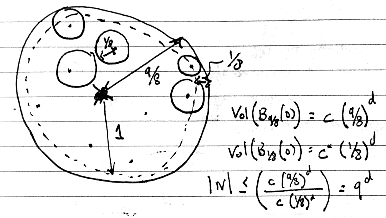
\includegraphics[width=0.6\textwidth]{figures/9-10-1.png}
        \caption{$1/8$-radius balls centered
            at all packing points are disjoint, the union of all these balls is contained in $B_{9/8}(0)$,
            so the cardinality $\lvert N \rvert \leq \left(\frac{9/8}{1/8}\right)^d = 9^d$.}
        \label{fig:9-10-1}
    \end{figure}
    
    Let $v \in \cS^{d-1}$ maximize $v^\top M v$
    and $u \in N$ such that $\|u - v\|_2 \leq \frac{1}{4}$.
    Such a $u$ must exist,
    otherwise $N \cup \{v\}$ is a larger $1/4$-packing which contradicts maximality of $N$.
    \begin{align}
        \|M\| - \lvert u^\top M u \rvert
        &= \lvert v^\top M v \rvert - \lvert u^\top M u \rvert \\
        &\leq \lvert v^\top M v - u^\top M u \rvert \\
        &= \lvert (u + v)^\top M (u - v) \rvert \\
        &\leq \underbrace{\|u + v\|_2}_{\leq 2} \|M\| \underbrace{\|u - v\|_2}_{\leq 1/4} \\
        &\leq \frac{1}{2} \|M\|
    \end{align}
    Hence $\|M\| \leq 2 u^\top M u \leq 2 \sup_{u \in N} u^\top M u$ as desired.
\end{proof}

\subsection{VC inequality and Symmetrization}

In this section, we will see how a family of events with certain geometric structure (which we will
quantify using VC-dimension) converges to its expectation at a rate dependent on the geometry.
In the process, we will encounter the technique of \emph{symmetrization}
(Prof. Steinhardt calls it ``bring your own randomness'') used to add additional randomness which
will be required to get concentration.

Let $\cH$ be a collection of functions $f : \cX \to \{0,1\}$ and $\{X_i \in \cX\}_{i=1}^n \simiid p$.
For $f \in \cH$, let
\begin{align}
    \nu(f) &= \ex_{x \sim p}[ f(x)] = \Pr_{x \sim p}[f(X) = 1] \\
    \nu_n(f) &= \frac{1}{n} \sum_{i=1}^n f(X_i) = \frac{1}{n} \#\{i : f(X_i) = 1\}
\end{align}
be the population and empirical averages respectively.

\textbf{Question}: How big is the discrepancy
\begin{align}
    D_n &= \sup_{f \in \cH} \lvert v_n(f) - v(f) \rvert
\end{align}

\textbf{Easy case}: $\lvert \cH \rvert < \infty$. Since $f(X_i)$ is bounded, apply \nameref{corr:hoeffding-inequality}
to the sum of independent bounded random variables to get:
\begin{align}
    D_n &= \max_{f \in \cH} \frac{1}{n} \sum_{i=1}^n (f(X_i) - \ex f(X)) \\
    \Pr\left[\frac{1}{n} \sum_{i=1}^n (f(X_i) - \ex f(X) \geq t \right] &\leq \exp(-2 n t^2)
\end{align}
A subsequent union bound over $\lvert \cH \rvert$ reveals
$t = O\left(\sqrt{\frac{1}{2n} \left( \log \lvert \cH \rvert + \log \frac{1}{\delta} \right)}\right)$

\textbf{More common case}: $\lvert \cH \rvert = \infty$. 
In this situation, we will bound $D_n$ using the geometry of $\cH$.
To do so, we will quantify the geometry using the following definitions:

\begin{definition}[Shattering number / VC dimension]
    The \emph{shattering number} of $\cH$ is
    \begin{align}
        V_{\cH}(\{x_i\}_{i=1}^n) &= \text{\# distinct} \{(f(x_1), \ldots, f(x_n)) : f \in \cH\} \\
        V_{\cH}(n) &= \max_{\lvert S \rvert = n} V_{\cH}(S)
    \end{align}
    It measures the number of possible ways to assign $\{0,1\}$ labels to $x_i$ which can be perfectly
    fit by $f \in \cH$.
    
    The \emph{VC dimension}
    \begin{align}
        vc(\cH) &= \max\{ n : V_{\cH}(n) = 2^n\}\label{eq:vc-dim-def}
    \end{align}
    It measures the largest cardinality $n$ such that for any set of points $S$ with cardinality $\lvert S \rvert = n$
    and any $\{0,1\}$ labelling of those points, some $f \in \cH$ can perfectly fit it.
\end{definition}

The shattering number is useful because instead of taking $\sup_{f \in \cH}$ of a term
involving $f$ only through $\{f(X_i)\}_{i=1}^n$, we can instead take the supremum over
$\{f(X_i)\}_{i=1}^n$ directly and only deal with $V_{\cH}(n)$ terms.

\begin{example}[VC dimension of half spaces]\label{eg:half-spaces-vc}
    Let $\cX = \RR^d$, $\cH = \text{half spaces} = \{f(x) = \ind[\braket{v,x} \geq \tau] : v \in \RR^d, \tau \in \RR \}$.
    Then $vc(\cH) = d+1$.
    
    We will see a proof next time, but for now consider an example where $d=2$.
    We can always separate 3 points by drawing a line, so $vc(\cH) \geq 3$.
    However, with 4 points there can be crossings (see \cref{fig:9-10-vc-hs}) which cannot be shattered.
        \begin{figure}[H]
        \centering
        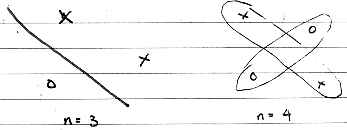
\includegraphics[width=0.6\textwidth]{figures/9-10-2.png}
        \label{fig:9-10-vc-hs}
        \caption{$n=3$ can always be shattered by a line, but the crossings possible when $n=4$ prevent this.}
    \end{figure}
\end{example}

Clearly by definition $V_\cH(n) = 2^n$ for all $n \leq vc(\cH)$.
When $n > vc(\cH)$, by \myref{eq:vc-dim-def} we have $V_\cH(n) < 2^n$.
The following lemma quantifies this and shows that the shattering number
is actually significantly smaller (growing polynomially in $n$ rather than exponentially):
\begin{lemma}[Sauer-Shelah]\label{lem:sauer-shelah}
    If $vc(\cH) = d$, then $V_{\cH}(n) \leq 2 n^d$.
\end{lemma}
While we will use this without proof, \nameref{lem:sauer-shelah} is the main reason why VC dimension
is useful for us: it allows us to convert the infinite supremum over $f \in \cH$ into a finite supremum over
$O(n^{\vc(\cH)})$ many terms of the form $\{f(X_i)\}_{i=1}^d$.

\begin{theorem}[VC inequality]\label{thm:vc-inequality}
    With probability $\geq 1 - \delta$
    \begin{align}
        D_n = O\left(\sqrt{\frac{vc(\cH) + \log \frac{1}{\delta}}{n}}\right)    
    \end{align}
\end{theorem}

\begin{proof}
    We will show something weaker, namely:
    \begin{align}
        \ex D_n &\leq O\left( \frac{vc(\cH) \log n}{n} \right)
    \end{align}
    The $\log \frac{1}{\delta}$ tail bound follows from McDarmid's inequality,
    and removing the extra $\log n$ refines the argument we will give using a tool called chaining.
    
    \textbf{Incorrect proof path}: Notice that
    \begin{align}
        D_n &= \sup_{f \in \cH} \left\lvert
            \underbrace{\frac{1}{n} \sum_{i=1}^n (f(X_i) - \ex f(X))}_{\Pr[\cdot \geq t] \leq \exp(-2 n t^2)}
        \right\rvert
    \end{align}
    So \nameref{corr:hoeffding-inequality} can be used to control the term inside the supremum.
    Let $vc(\cH) = d$.
    By \cref{lem:sauer-shelah}, there are only $O(n^d)$ distinct $(f(X_1), \ldots, f(X_n))$
    so a union bound implies $t = O\left(\sqrt{\frac{d \log n + \log \frac{1}{\delta}}{2n}}\right)$
    
    This is incorrect because applying Sauer-Shelah requires us to condition on a specific realization of $\{X_i\}_{i=1}^n$
    (after which we know there are at most $V_{\cH}(n)$ distinct values of $(f(X_1), \ldots, f(X_n))$).
    After conditioning, there's no randomness left for applying \nameref{corr:hoeffding-inequality} to get concentration.
    
    \textbf{Solution}: Introduce additional randomness using \emph{symmetrization}.
    Introduce independent copies $X_i'$ and note
    \begin{align}
        \ex[D_n] &= \ex_{X_1, \ldots, X_n}\left[\sup_{f \in \cH} \left\lvert
            \frac{1}{n} \sum_{i=1}^n f(X_i) - \ex f(X)
        \right\rvert \right] \\
        &= \ex_{X_1, \ldots, X_n} \left[ \sup_{f \in \cH} \left\lvert \ex_{X_1', \ldots, X_n'} \left[
            \frac{1}{n} \sum_{i=1}^n (f(X_i) - f(X_i'))
        \right]\right\rvert\right]
    \end{align}
    $\lvert \cdot \rvert$ is convex, so by Jensen's inequality
    \begin{align}
        \ex[D_n]
        \leq \ex_{X} \left[ \sup_{f \in \cH} \ex_{X'} \left[\left\lvert 
            \frac{1}{n} \sum_{i=1}^n (f(X_i) - f(X_i'))
        \right\rvert \right]\right]
    \end{align}
    Also, $\sup_y \ex f(X,y) \leq \ex \sup_y f(X,y)$ for any function $f$ 
    (since $\ex f(X,y) \leq \ex \sup_y f(X,y)$ then take supremum on left-hand side, or see Fatou-Lebesgue theorem)
    hence we can move $\ex_{X'}$ out of $\sup_{f \in \cH}$ to get
    \begin{align}
        \ex[D_n]
        &\leq \ex_{X, X'}\left[
        \sup_{f \in \cH} \left\lvert \frac{1}{n} \sum_{i=1}^n ( f(X_i) - f(X_i') ) 
        \right\rvert\right]
    \end{align}
    Here is where the randomness from symmetrization is added:
    since $f(X_i) - f(X_i') \overset{d}{=} \eps_i(f(X_i) - f(X_i'))$ for $\eps_i \sim \text{Rad}$
    \begin{align}
        \ex[D_n]
        &\leq \ex_{X, X', \eps}\left[
        \sup_{f \in \cH} \left\lvert \frac{1}{n} \sum_{i=1}^n \eps_i ( f(X_i) - f(X_i') ) 
        \right\rvert\right] \label{eq:9-10-symmetrized-need-concentration}
    \end{align}
    Condition on $X, X'$ and let $f(X_i) = a \in V_{\cH}(\{x_1, \ldots, x_n\})$
    and $f(X_i') = b \in V_\cH(\{x_1', \ldots, x_n'\})$. Then
    \begin{align}
        \sup_{f \in \cH}
            \left\lvert \frac{1}{n} \sum_{i=1}^n \eps_i(f(X_i) - f(X_i')) \right\rvert
        &= \sup_{a, b} 
            \underbrace{
                \left\lvert \frac{1}{n} \sum_{i=1}^n \eps_i (a_i - b_i)\right\rvert
            }_{\Pr[\lvert \cdot \rvert \geq t] \leq 2 \exp(\frac{-n t^2}{2})}
    \end{align}
    Now we can apply \nameref{corr:hoeffding-inequality} (picking up an extra factor of $2$ because
    of the absolute value, see \cref{eq:tail-bound-abs-value-two-factor}) to the independent,
    zero-mean (since $\ex \eps_i = 0$),
    bounded (since $a_i$, $b_i$, and $\eps_i$ are all bounded)
    random (since $\eps_i$ is still random) variables
    and union bound over the $O(n^{2d})$ (by \nameref{lem:sauer-shelah}, squared since there is both $f(X)$ and $f(X')$) distinct $f(X)$ and $f(X')$
    \begin{align}
        \Pr\left[ \sup_{f \in \cH}
            \left\lvert \frac{1}{n} \sum_{i=1}^n \eps_i(f(X_i) - f(X_i')) \right\rvert \geq t 
        \middle| X, X' \right]
        &\leq (2 n^{2d}) 2 \exp\left(\frac{-n t^2}{2} \right) \\
    \end{align}
    This tail probability is small if $t \gg \sqrt{\frac{d \log n}{n}}$, so \todo{why?? Try $\ex X = \int P(X \geq t) dt$ for $X \geq 0$}
    the expectation over $\eps$ in \cref{eq:9-10-symmetrized-need-concentration} is of the same order
    and we have
    \begin{align}
        \ex[D_n]
        &\leq \ex_{X, X'}\left[
            \ex_{\eps}\left[
                \sup_{f \in \cH} \left\lvert \frac{1}{n} \sum_{i=1}^n \eps_i ( f(X_i) - f(X_i') ) 
                \middle| X, X'\right]
        \right\rvert\right]
        = O\left(
            \sqrt{\frac{d \log n}{n}}
        \right)
    \end{align}
\end{proof}

Discretization to a representative set (``fingerprinting'') is how previous sections worked.
The complication here is that to apply \cref{lem:sauer-shelah} we had to condition on $X_i$ and
remove the randomness. The secret sauce was to add randomness back using the $\eps_i$ in
symmetrization.
\section{9/12/2019}

\subsection{Recap}

\begin{itemize}
    \item Bounded $\ex \sup_{v \in V} X(v)$ where $X(v)$ concentrates
        and $V$ is finite or could be well approximated by a finite set
        \begin{itemize}
            \item Top eigenvalue of random covariance matrix
            \item VC inequality and symmetrization
        \end{itemize}
    \item Debt: VC-dim of halfspaces is $d+1$ (\cref{eg:half-spaces-vc})
\end{itemize}
Today, we will:
\begin{itemize}
    \item Pay off debt: prove the VC dimension of half spaces is $d+1$
    \item Give a finite-sample analysis of \myref{def:mdf}
    \begin{itemize}
        \item Weaken $\TV$ to $\widetilde{\TV}$
        \item Bound \nameref{prop:mdf-modulus-error-bound} via ``mean crossing lemma''
        \item $\widetilde{\TV}(\tilde{p}, \tilde{p}_n) \to 0$ as $n \to \infty$
    \end{itemize}
\end{itemize}

\subsection{VC dimension of half spaces}

In \myref{eg:half-spaces-vc} we claimed that $vc(\cH) = d+1$ for
the family of half spaces (i.e. linear decision boundaries)
\begin{align}
    \cH = \{ \ind\{\braket{v,x} \geq \tau\} : v \in \RR^d, \tau \in \RR\}
\end{align}
We previously showed it geometrically for the case when $d=2$.
Here, we will generalize this to higher dimensions.

\begin{proposition}[VC dimension of half spaces]\label{prop:vc-dim-half-spaces}
    No $d+2$ set of points in $\RR^d$ can be shattered by any $f \in \cH$.
\end{proposition}

\begin{proof}
    Fix $\{x_i\}_{i=1}^{d+2} \in \RR^d$ distinct.
    We will find two sets $S_+, S_- \subset \{x_1, \ldots, x_{d+2}\}$ such
    that $S_+ \cap S_- = \emptyset$ but $\conv(S_+) \cap \conv(S_-) \neq \emptyset$.
    This is sufficient because every $f = \ind\{\braket{v,x} \geq \tau\} \in \cH$
    can be identified with a half-space (of the points classified $+1$ by $f$)
    \begin{align}
        H = f^{-1}(\{1\}) = \{ x \in \RR^d : \braket{v,x} \geq \tau \}
    \end{align}
    and by convexity of $H$
    \begin{align}
        S_+ \subset H &\implies \conv(S_+) \subset H
    \end{align}
    Hence, if $f$ correctly classifies all of $S_+$ then it must also
    misclassify some $x \in S_+ \cap S_- \subset S_-$.

    Consider the linear system
    \begin{align}
        \sum_{i=1}^{d+2} a_i x_i = 0, \qquad \sum_{i=1}^{d+2} a_i = 0
        \label{eq:9-12-lin-system}
    \end{align}
    or equivalently in matrix form
    \begin{align}
        \underbrace{\begin{bmatrix}
            \vdots & \vdots & \hdots & \vdots \\
            x_1 & x_2 & \hdots & x_{d+2} \\
            \vdots & \vdots & \hdots & \vdots \\
            1 & 1 & \hdots & 1
        \end{bmatrix}}_{(d+1) \times (d+2)} \begin{bmatrix}
            a_1 \\ \vdots \\ a_{d+2}
        \end{bmatrix} = \vec{0}
    \end{align}
    By the rank-nullity theorem, the null-space must have dimension $\geq 1$
    hence there exists at least one solution $\vec{a}$.
    Let
    \begin{align}
        S_+ = \{ i : a_i > 0 \}, \qquad S_- = \{ i : a_i < 0 \}
    \end{align}
    Then by \cref{eq:9-12-lin-system}
    \begin{align}
        \underbrace{\sum_{i \in S_+} \underbrace{\frac{a_i}{A}}_{\in [0,1]} x_i}_{\in \conv(S_+)}
        = \underbrace{\sum_{i \in S_-} \underbrace{\frac{a_i}{A}}_{\in [0,1]} x_i }_{\in \conv(S_-)}
        \qquad \text{where} \quad A = \sum_{i \in S_+} a_i = \sum_{i \in S_-} (-a_i)
    \end{align}
    This gives us a point in $\conv(S_+) \cap \conv(S_-)$.
\end{proof}

\begin{remark}
    The geometric result that ``any set of $d+2$ points in $\RR^d$ can be
    partitioned into two disjoint sets whose convex hulls intersect'' is known
    as \emph{Radon's theorem} on convex sets.
\end{remark}

\subsection{Finite sample analysis of MDF via Generalized KS distance}

Recall \myref{def:mdf} projects $\tilde{p}$ on to $\cG$ under some discrepancy
$D$.  Previously we worked with $D = \TV$, which works fine if $\tilde{p}$ is a
continuous distribution (e.g. $\tilde{p} = \cN(\mu, I)$ in \cref{lem:gauss-tv}).
However, when we only have a finite number of samples we can only form the
empirical distribution
\begin{align}
    \tilde{p}_n
    &= \frac{1}{n} \sum_{i=1}^n \delta_{X_i},
    \qquad X_i \sim \tilde{p}
\end{align}
Here, $\TV$ is inadequate because $\TV(\tilde{p}_n, p) = 1$ almost surely
for any continuous distribution $p$ (this is because $\Pr_{X \sim p}[X = X_i] = 0$)
so it's not clear how to project onto a continuous family such as $\cG_{gauss}$.
Moreover, in many cases $\TV(\tilde{p}_n, \tilde{p}) = 1$ even as $n \to \infty$.

To address this issue, we can consider relaxing $\TV$ to
a weakening $\widetilde{\TV}$ which is more forgiving.
We have two desidirata for $\widetilde{\TV}$:
\begin{enumerate}
    \item The modulus $\fm(\cG, \eps, \widetilde{\TV})$ remains small, so that
        \myref{prop:mdf-modulus-error-bound} still gives a good result
    \item $\widetilde{\TV}(\tilde{p}, \tilde{p}_n) \to 0$ as $n \to \infty$,
        so that $\widetilde{\TV}$ detects convergence of (discrete) empirical
        distributions to a (possibly continuous) population distribution
\end{enumerate}

\begin{remark}
    The two desidirata are competing.
    We want $\widetilde{\TV}$ to be large in
    (1) so that $A = \{ (p,q) \in \cG : \widetilde{\TV}(p,q) \leq \eps \}$ is
    small and hence $\fm = \sup_{(p,q) \in A} L(p, \theta^*(q))$ is small.
    At the same time, in (2) we would like $\widetilde{\TV}$ to be small
    to avoid the failure of $\TV$ in detecting $\tilde{p_n} \to \tilde{p}$
    (e.g. Glivenko-Cantelli ensures that the cumulative distribution functions
    converge uniformly).
\end{remark}

\begin{proposition}\label{prop:mdf-tilde-tv}
    Suppose $\tilde{\TV}$ is a pseudometric such that
    $\widetilde{\TV} \leq \TV$. Let $\hat{\theta}_{\widetilde{\TV}}(p) = \theta^*(q)$ where
    $q \in \argmin_{q \in \cG} \widetilde{\TV}(p, q)$ (the \nameref{def:mdf}
    under $\widetilde{\TV}$). Then
    \begin{align}
        L(p^*, \hat{\theta}_{\widetilde{\TV}}(\tilde{p}_n))
        &\leq \fm(\cG, 2 \eps', \widetilde{\TV})
    \end{align}
    where $\eps' = \eps + \widetilde{\TV}(\tilde{p}, \tilde{p}_n)$
    (and $\widetilde{\TV}(p^*, \tilde{p}) \leq \eps$ as per the conventions
    outlined in \cref{fig:robust-statistics-framework})
\end{proposition}

\begin{proof}
    By \myref{prop:mdf-modulus-error-bound}
    \begin{align}
        L(p^*, \hat{\theta}_{\widetilde{\TV}}(\tilde{p}_n))
        &\leq \fm(\cG, 2 \widetilde{\TV}(p^*, \tilde{p}_n), \widetilde{\TV}, L)
    \end{align}
    Since $\widetilde{\TV}$ is a pseudometric, by the triangle
    inequality
    \begin{align}
        \widetilde{\TV}(p^*, \tilde{p}_n)
        &\leq \underbrace{\widetilde{\TV}(p^*, \tilde{p})}_{\leq \eps} + \widetilde{\TV}(\tilde{p}, \tilde{p}_n)
    \end{align}
\end{proof}

How do we construct $\widetilde{\TV}$?
\begin{definition}[Generalized Kolmogorov-Smirnov distance]\label{def:tilde-tv}
    For a family of functions $\cH = \{ f : \cX \to \RR \}$,
    the \emph{generalized Kolmogorov-Smirnov distance}
    induced by $\cH$ is
    \begin{align}
        \widetilde{\TV}_{\cH}(p, q) &= \sup_{f \in \cH, \tau \in \RR}
        \left\lvert \Pr_p[f(X) \geq \tau] - \Pr_q[f(X) \geq \tau] \right\rvert
    \end{align}
\end{definition}

\begin{remark}
    For $f \in \cH$ and $\tau \in \RR$, if we define the event
    $E_{f,\tau} = \{f(X) \geq \tau\}$ then notice
    \begin{align}
        \widetilde{\TV}_\cH(p,q)
        = \sup_{E_{f,\tau}} \left\lvert
            \Pr_p[E_{f,\tau}] - \Pr_q[E_{f,\tau}]
        \right\rvert
        &\leq \sup_{E~\text{meas}} \left\lvert
            \Pr_p[E] - \Pr_q[E]
        \right\rvert
        = \TV(p,q)
    \end{align}
    So $\widehat{\TV}$ is indeed dominated by $\TV$ as required by
    \cref{prop:mdf-tilde-tv}.
\end{remark}


What $\cH$ should we pick? The answer depends on what we are trying to estimate
(i.e. choice of $L(p, \theta)$). For now, consider mean estimation
(i.e. $L(p,\theta) = \|\theta - \mu(p)\|_2$).
One intuition is that knowledge of the one dimensional
projections ($\ex\braket{v,x}$ for all $v \in \RR^d$) allows us to know
$\ex[X]$, so it's reasonable to consider
\begin{align}
    \cH = \cH_{lin} = \{ x \mapsto \braket{v, x} : v \in \RR^d \}
\end{align}

To bound the modulus, recall that previously if $p, q \in \cG_{\TV}$ are
\nameref{def:resilience}s then \cref{corr:mod-bound-resilient} gave us
\begin{align}
    \TV(p, q) \leq \eps &\implies \|\mu(p) - \mu(q)\|_2 \leq 2 \rho
\end{align}
Similarly, here we will also restrict our distributional assumptions to
be within resilient distributions: $\cG \subset \cG_{\TV}$.

We need to show our two desidirata:
\begin{enumerate}
    \item The modulus is bounded:
    \begin{align}
        p,q \in \cG \subset \cG_{\TV}(\rho, \eps)
        \text{ and } \widetilde{\TV}(p,q) \leq \eps
        \implies \|\mu(p) - \mu(q)\|_2 \leq \sigma = 2 \rho\label{eq:9-12-desidirata-1}
    \end{align}
    \item $\widetilde{\TV}(\tilde{p}, \tilde{p}_n)$ is small, specifically:
    \begin{align}
        \widetilde{\TV}(\tilde{p}, \tilde{p}_n) = O\left(\sqrt{d/n}\right)\label{eq:9-12-desidirata-2}
    \end{align}
\end{enumerate}

\begin{proof}[Proof of \cref{eq:9-12-desidirata-1}]
    Previously we used \nameref{lem:midpoint} to find an $\eps$-deletion
    $r \leq \min\left\{\frac{p}{1 - \eps}, \frac{q}{1 - \eps}\right\}$
    close to both $p$ and $q$ in the sense that
    \begin{align}
            \| \mu(p) - \mu(r) \|_2 \leq \rho
            \text{ and }
            \|\mu(q) - \mu(r) \|_2 \leq \rho
    \end{align}
    After which a triangle inequality completed the proof.

    Unfortunately, we don't know of a way to find a single midpoint distribution
    under $\widetilde{\TV}$.  Instead, we will use the following key property:

    \begin{lemma}[Mean crossing property]\label{lem:mean-crossing-property}
        Suppose $\widetilde{\TV}(p,q) \leq \eps$.
        For any $v \in \RR^d$, there exists $\eps$-deletions $r_p \leq \frac{p}{1 - \eps}$ and $r_q \leq \frac{q}{1 - \eps}$ such that
        \begin{align}
            \ex_{r_q} \braket{v,x} \leq \ex_{r_p} \braket{v,x}
        \end{align}
        In other words, after deleting $\eps$ mass to create $r_q$ and $r_p$, the
        means are shifted such that they cross.
    \end{lemma}

    If we have the $\epsilon$ deletions
    $r_p \leq \frac{p}{1 - \eps}$ and $r_q \leq \frac{q}{1 - \eps}$ from
    \myref{lem:mean-crossing-property}, then
    \begin{align}
        \underbrace{\ex_p \braket{v,x}}_{=\braket{v, \mu_p}}
        &\leq \ex_{r_p}[\braket{v,x}] + \rho &&\text{resilience of $p$} \\
        &\leq \ex_{r_q}[\braket{v,x}] + \rho &&\text{mean crossing} \\
        &\leq \underbrace{\ex_{q}[\braket{v,x}]}_{=\braket{v, \mu_q}} + 2\rho &&\text{resilience of $q$}
    \end{align}
    Hence
    \begin{align}
        \braket{v, \mu_p - \mu_q}
        &\leq 2 \rho
    \end{align}
    for all $\|v\|_2 = 1$. Therefore $\|\mu_p - \mu_q\|_2 \leq 2 \rho$.
\end{proof}

\begin{figure}[H]
    \begin{center}
        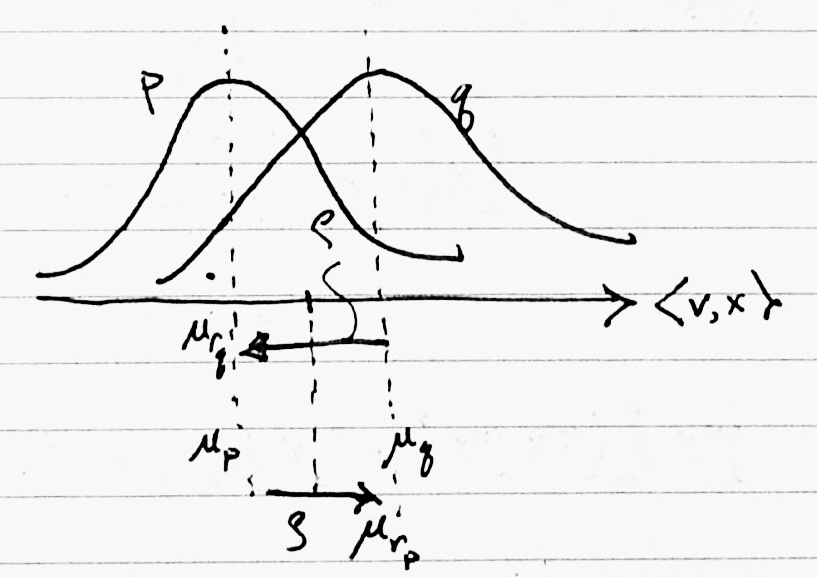
\includegraphics[width=0.4\textwidth]{figures/9-12-1.png}
    \end{center}
    \caption{
        Resilience allows us to perform an $\eps$-deletion to
        move from $\mu_p \to \mu_{r_p}$ and $\mu_q \to \mu_{r_q}$
        and pick up a factor of $+2 \rho$.
        Mean crossing allows us to relate $\mu_{r_p}$ and $\mu_{r_q}$.
    }
    \label{fig:resilience-mean-crossing}
\end{figure}

\begin{proof}[Proof of \nameref{lem:mean-crossing-property}]
    Consider \cref{fig:resilience-mean-crossing}, which visualizes the 1D
    projections of $p$ and $q$ in the $v$ direction.  To make $\braket{v,
    \mu_{r_q}}$ cross over $\braket{v, \mu_{r_p}}$, we would like to shift the
    mean of $q$ to the left and the mean of $p$ to the right as much as
    possible.  Thus, delete $\eps$ mass from the right tail of $q$ (and delete
    the left tail of $p$). Then
    \begin{align}
        \Pr_{r_p}[\braket{v,x} \geq \tau]
        \geq \frac{\Pr_{p}[\braket{v,x} \geq \tau]}{1 - \eps}
        \geq \frac{\Pr_{q}[\braket{v,x} \geq \tau] - \eps}{1 - \eps}
        = \Pr_{r_q}[\braket{v,x} \geq \tau]
    \end{align}
    where the first inequality is because $r_p$ is $p$ with the left
    tail deleted and renormalized by $1-\eps$,
    the second from
    $\Pr_q[\braket{v,x} \geq \tau] - \Pr_p[\braket{v,x} \geq \tau] \leq \widetilde{\TV}(p,q) \leq \eps$,
    and the third from $r_q$ being formed by deleting $\eps$ from the right tail of
    $q$ and renormalizing by $1-\eps$.

    We have shown that the right tail probabilities of $r_p$ are always larger
    than those of $r_q$, i.e. $r_p$ \emph{stochastically dominates} $r_q$.
    As a consequence, $\ex_{r_p}[\braket{v,x}] \geq \ex_{r_q}[\braket{v,x}]$.
\end{proof}

\begin{proof}[Proof of \cref{eq:9-12-desidirata-2}]
    Notice
    \begin{align}
        \widehat{\TV}_{\cH_{\lin}}(p,q)
        &= \sup_{v \in \RR^d, \tau \in \RR} \left\lvert
            \underbrace{\Pr_p[\braket{v,x} \geq \tau] - \Pr_q[\braket{v,x} \geq \tau]}_{\text{max discrepancy on halfspaces}}
        \right\rvert
    \end{align}
    By \nameref{thm:vc-inequality} and \myref{prop:vc-dim-half-spaces}
    \begin{align}
        \widehat{\TV}_{\cH_{\lin}}(\tilde{p}, \tilde{p}_n)
        &\leq O\left(\sqrt{\frac{vc(\text{half spaces})}{n}}\right)
        = O\left(\sqrt{\frac{d + \log \frac{1}{\delta}}{n}}\right)
    \end{align}
    with probability $\geq 1 - \delta$.
\end{proof}

\textbf{Consequences}:
\begin{itemize}
    \item For $(\rho, \eps + O(\sqrt{d/n}))$-resilient distributions, we can estimate mean with error $2 \rho$
    \item For bounded covariance, \cref{corr:mod-cont-cov} gave us
        $\rho(\eps) = O(\sqrt{\eps})$ hence
    \begin{align}
        L(p^*, \tilde{\theta}_{\widetilde{\TV}}(\tilde{p}_n)) 
        \leq O\left(\sqrt{\eps + \sqrt{d/n}}\right)
    \end{align}
    The lower bound $\sqrt{\eps}$ is what we get in the infinite sample $n \to \infty$
    limit, and $\sqrt{d/n}$ when $\eps \to 0$, so we would like $\sqrt{\eps} + \sqrt{d/n}$.
    The slack in the bound comes from $n \gg d / \eps^2$, whereas we would need $n \gg \frac{d}{\eps}$ but this analysis doesnt give it to us.

    \item For sub-Gaussians, $\rho(\eps) = O(\eps \sqrt{\log(1/\eps)})$.
    When $n \gg \frac{d}{\eps^2}$ we get $O(\eps \sqrt{\log (1/\eps)}$.
\end{itemize}
In general, this analysis holds for $n \gg d / \eps^2$: whenever this holds, we can
do as well as if we had infinite data. The analysis is tight in $d$ but loose in $\eps$.

\todo{$\widetilde{\TV}$ similar to Tukey median, may be useful for challenge problem}


\bibliography{refs.bib}

\end{document}
